\chapter{Fundamentação Teórica}

% TODO: Atualizar isso aqui
Neste capítulo serão discutidos os aspectos relacionados à classificação de imagens de lesões de pele e detecção de melanomas. Além disso, serão explicados os conceitos
de visão computacional com redes neurais, \acp{LLM} e como estas tecnologias se integram em um \ac{MLLM}. Por fim, será discutido sobre diferentes métodos de
\textit{fine-tuning}.

\section{Lesões de Pele}

A pele é o maior órgão do corpo humano e é responsável por proteger o corpo de agentes microbiológicos, físicos e químicos. Além disso, ela também ajuda na regulação da
temperatura do corpo e, através de receptores cutâneos, proporciona informações sensoriais como o tato \cite{skin}.

Devido à exposição da pele ao ambiente, é mais comum que esse órgão sofra com doenças. As áreas afetadas são consideradas lesões de pele e podem ser usadas para
diagnósticos \cite{segmentation_skin_lesions}.

\subsection{Câncer de Pele}

O câncer é uma doença caracterizada pela multiplicação de células anormais que podem se espalhar para além do seu tecido de origem, causando tumores e levando
eventualmente à morte \cite{cancer}. O câncer de pele é o tipo mais comum da doença globalmente e é mais frequentemente causado pela exposição prolongada à radiação
ultravioleta \cite{skin_cancer}. Em geral, essa doença afeta mais a pele clara e pode afetar a mesma pessoa mais de uma vez. Uma vez desenvolvido, há um aumento de 35\%
no risco de desenvolvimento de um novo câncer de pele do mesmo tipo em um período de três anos \cite{skin_cancer_zink}.

Existem várias categorias de câncer de pele, elas podem ser agrupadas como \ac{CPNM} e melanoma. \ac{CPNM} podem ser subdivididos em \ac{CBC}, \ac{CEC}, carcinoma de
Merkel e entre outros. Essa categoria é a mais incidente, correspondendo a mais de 90\% dos cânceres diagnosticados e também é a menos fatal. O subtipo \ac{CBC} é o
mais frequente e corresponde a mais de 75\% dos casos de \ac{CPNM} no Brasil \cite{skin_cancer_zink}. O melanoma é o tipo mais fatal e menos incidente da doença. Cerca
de 75\% das mortes por câncer de pele são causadas por melanomas \cite{skin_cancer_screening}.

A doença tem um prognóstico muito melhor quando a detecção e tratamento são feitos cedo o suficiente. Segundo \textcite{skin_cancer_survival}, a taxa de sobrevivência ao
melanoma no Brasil é menor que a taxa global, sendo que há uma prevalência maior de casos avançados.

\subsection{Imagens de Lesões de Pele}

As imagens para exames dermatológicos podem ser agrupadas em diferentes categorias. Alguns exemplos baseados em procedimentos recomendados por
\textcite{fotos_dermatologia} são:

% TODO: Adicionar imagens

\begin{itemize}
      \item \textbf{Dermatoscopia}: Essas imagens são obtidas com um equipamento especializado, o dermatoscópio. Esse método permite que um diagnóstico mais preciso seja
            feito, sendo melhor que o olho nu na detecção de melanomas \cite{dermatoscopy}.
      \item \textbf{Foto de aproximação com régua}: Esse tipo de imagem é obtida com uma fotografia feita a 30 centímetros da lesão, sem utilizar \textit{zoom}.
            Nessas imagens, etiquetas são colocadas próximas à lesão para auxiliar na determinação do seu tamanho.
      \item \textbf{Foto panorâmica}: Nesse método são registradas imagens de regiões do corpo, como da cabeça, tronco, braços e pernas.
\end{itemize}

\subsection{Detecção e Diagnóstico de Câncer de Pele}

O câncer de pele pode ser identificado e classificado através dos sintomas causados. Características como o tamanho da lesão, variação da cor, irregularidade do formato,
progresso ao longo do tempo e local do corpo em que a lesão se encontra são fundamentais para o diagnóstico da doença \cite{recognizing_skin_cancer}.

A análise destes sintomas é normalmente um processo visual realizado por um dermatologista, sendo que técnicas como a dermatoscopia e teledermatologia podem ser usadas.
Outros métodos não invasivos incluem, por exemplo, a análise intracutânea espectrofotométrica, ultrasonografia de alta frequência e microscopia confocal de refletância.
É possível também diagnosticar a doença através de métodos invasivos como a biópsia. Além destes métodos, há também a utilização de \ac{IA}. Soluções com \ac{IA}
utilizam imagens para a classificação da doença e podem ter uma precisão equiparável ou até maior a de dermatologistas \cite{recognizing_skin_cancer, skin_cancer_ai}.

\section{Multimodal Large Language Models}

\acp{MLLM} são \acp{IA} baseadas em \acp{LLM} que possuem a capacidade de interpretação de diferentes modalidades de informação, diferentemente de \acp{LLM}, que
operam sobre informações textuais. Esses modelos também podem ser capazes de produzir conteúdo multimodal. Essas modalidades podem ser imagens, vídeos, áudios e
entre outros \cite{mllm_survey_2023, mllm_survey_2024}.

Segundo \textcite{mllm_survey_2024}, a estrutura de um \ac{MLLM} pode ser dividida em cinco componentes, sendo eles o codificador de modalidade, projetor de entrada,
\ac{LLM}, projetor de saída e o gerador de modalidade. No caso de \acp{MLLM} que possuem apenas saída de texto, somente os três primeiros componentes estão presentes,
essa estrutura é demonstrada na \autoref{fig:mllm_structure_encoder_only}.

\begin{figure}[ht]
      \centering
      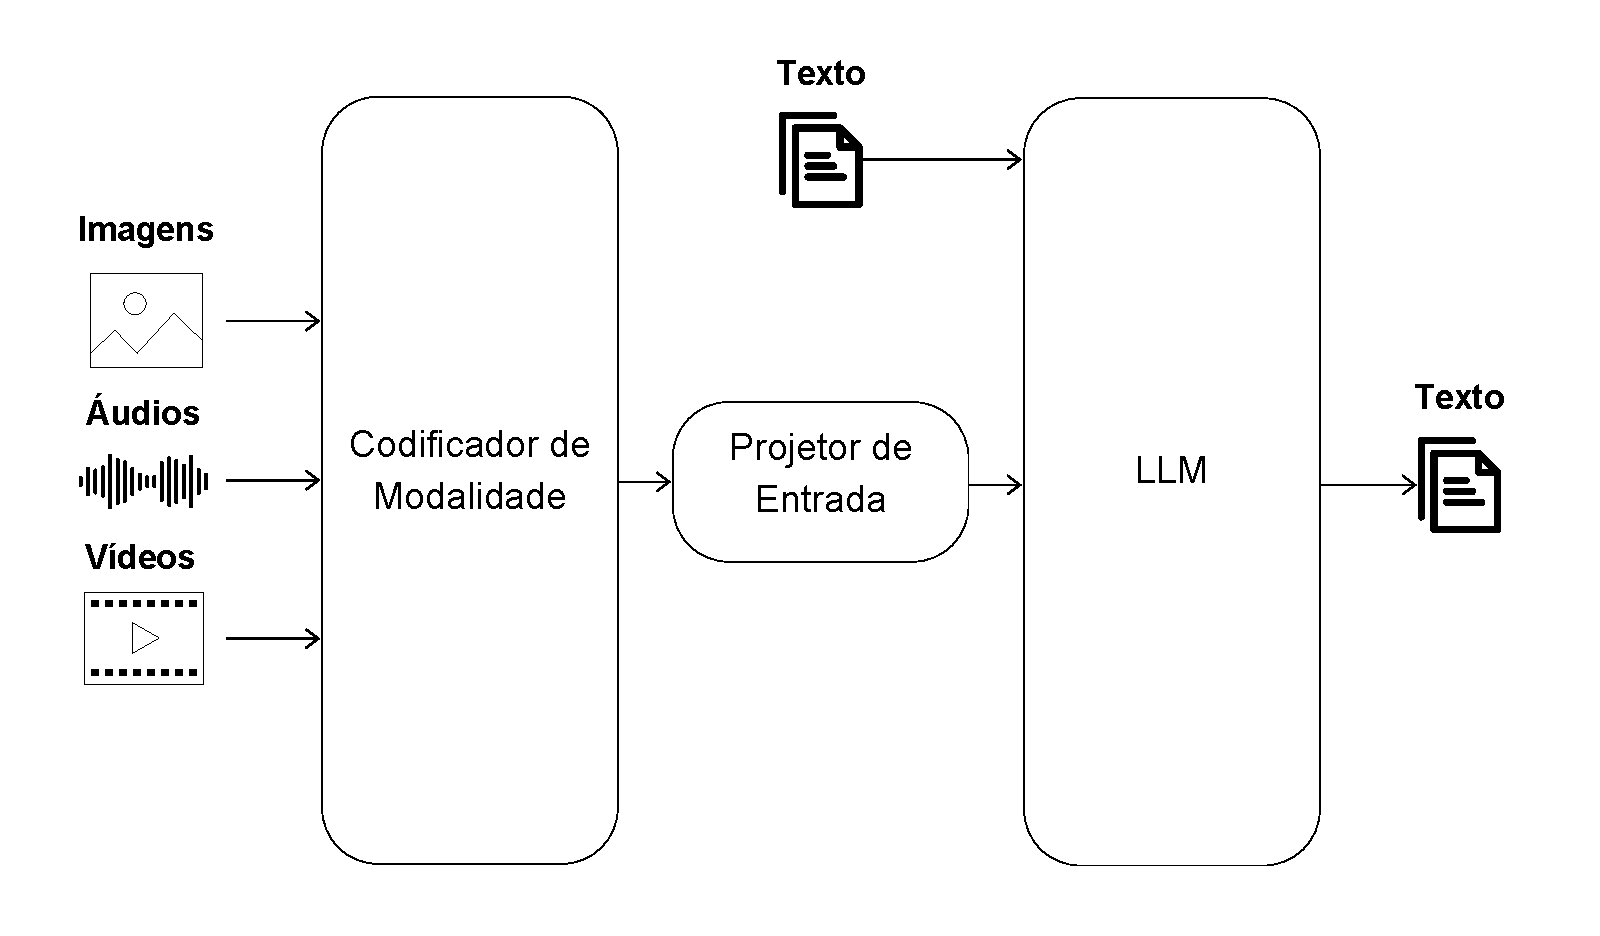
\includegraphics[width=0.7\columnwidth,keepaspectratio]{images/mllm_structure_encoder_only.pdf}
      \caption{\small Estrutura de um \ac{MLLM} que realiza apenas a interpretação multimodal.}
      \label{fig:mllm_structure_encoder_only}
\end{figure}

Neste trabalho, o foco será dado a modelos que interpretam imagens e retornam saídas textuais. Sendo assim, a parte de geração multimodal não será coberta.

\subsection{Large Language Models}

\acp{LLM} ou Grandes Modelos de Linguagem são modelos estatísticos pré-treinados baseados em transformadores capazes de processar e gerar textos em linguagem natural.

\subsubsection{Transformadores}

\subsubsubsection{Incorporação Vetorial}

Um \textit{embedding vector} ou uma incorporação vetorial é um vetor de valores reais em um espaço semântico n-dimensional que representa um dado, como, por exemplo, uma
palavra ou uma imagem. Esse tipo de representação permite que diferentes tipos de dados sejam representados em um espaço vetorial unificado. Na
\autoref{fig:word_embeddings} há um exemplo simplificado da estrutura destes vetores \cite{word_embedding, mllm_survey_2023}.

\begin{figure}[ht]
      \centering
      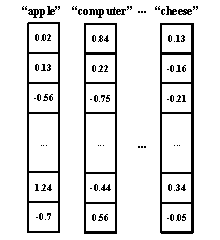
\includegraphics[width=0.4\columnwidth,keepaspectratio]{images/word_embeddings.pdf}
      \caption{\small Representação de palavras como vetores de valores reais. Fonte: \textcite{word_embedding}.}
      \label{fig:word_embeddings}
\end{figure}

Nesse espaço vetorial, direções podem ter um significado semântico. Um exemplo dado por \textcite{glove} demonstra isso com uma frase, traduzida do inglês: "Um rei é para
uma rainha o que um homem é para uma mulher", que pode ser representada como \textit{$V_{rei} - V_{rainha} \approx V_{homem} - V_{mulher}$}, evidenciando que a direção do
vetor \textit{$V_{rei} - V_{rainha}$} codifica informações sobre gênero. Além disso, a proximidade entre incorporações indica a similaridade semântica entre elas. Mais
exemplos dessa relação entre palavras podem ser vistos na \autoref{fig:word_embeddings_directions}.

\begin{figure}[ht]
      \centering
      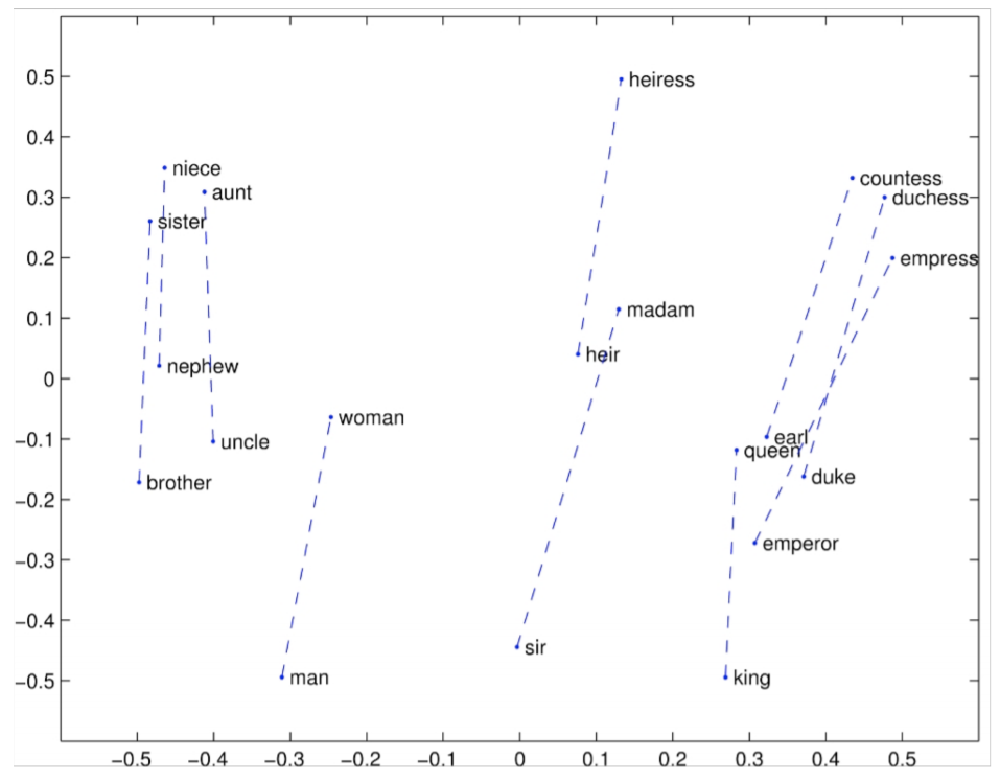
\includegraphics[width=0.7\columnwidth,keepaspectratio]{images/word_embeddings_directions.png}
      \caption{\small Visualização de incorporações com a direção que codifica informações de gênero evidenciada. Fonte: \textcite{word_embedding}.}
      \label{fig:word_embeddings_directions}
\end{figure}
\clearpage  % TODO: Apagar isso aqui se possível

\subsection{Codificador de Modalidade}

Codificadores de modalidade são os componentes responsáveis pela extração das características mais relevantes dos dados multimodais de entrada em incorporações vetoriais.
\cite{mllm_survey_2024}.

\subsubsection{Codificador Visual}

Existem diversos tipos de codificadores visuais. Os mais comuns usam \acp{ViT} ou Transformadores Visuais na suas arquiteturas, mas também há também codificadores
baseados em convolução \cite{mllm_survey_2023}. Neste trabalho o foco será direcionado a arquiteturas baseadas em \ac{ViT}.

\subsubsubsection{Transformadores Visuais}

\subsection{Projetor de Entrada}

\section{Fine-tuning}

\section{LLaMA}
